\documentclass{beamer}
\usepackage[utf8]{inputenc}
\usepackage[T1]{fontenc}
\usepackage{lmodern}
\usepackage{graphicx}
\usepackage{soul}
\usepackage{amsmath, amssymb}
\usepackage{fancyvrb}
\usepackage{color}
\usepackage{listings}
\lstset{
  escapeinside={<@}{@>},
  basicstyle=\ttfamily,
  columns=fullflexible,
  keepspaces=true,
}
\title{Zippers and Derivatives}
\author{Shuwei Hu}
%\institute{Technische Universität München}
\date{\today}

\DeclareMathOperator{\Flist}{\textbf{list}}
\DeclareMathOperator{\Fdlist}{\textbf{list\_context}}
\DeclareMathOperator{\Ftree}{\textbf{tree}}
\DeclareMathOperator{\Fdtree}{\textbf{tree\_context}}
\DeclareMathOperator{\Fbtree}{\textbf{btree}}
\DeclareMathOperator{\Fdbtree}{\textbf{btree\_context}}
\DeclareMathOperator{\Fltree}{\textbf{ltree}}
\DeclareMathOperator{\Fdltree}{\textbf{ltree\_context}}
\DeclareMathOperator{\Pa}{\frac{\partial}{\partial a}}

\begin{document}

\frame{\titlepage}

\section{Overview}

\begin{frame}
\frametitle{Overview}

\begin{itemize}
\item Zipper = context type, which helps moving through and ``modifying'' a functional data structure
\item Deriving context types vs.\ differentiating real-valued functions
\item Relation with combinatorial species
\end{itemize}
\end{frame}
\section{Zipper Examples}

%%%% begin [list] %%%%
\begin{frame}[fragile, allowframebreaks]
\frametitle{Zipper for List}

\begin{itemize}
\item \lstinline.datatype 'a list = Nil | Cons 'a ('a list).

\item How to define a "pointer" \lstinline|p| into a list \lstinline|l|, supporting:
\begin{itemize}
	\item \lstinline|p = begin(l)|
	\item \lstinline|p->prev|
	\item \lstinline|p->next|
	\item \lstinline|*p := a|
\end{itemize}
\end{itemize}

\framebreak

\begin{itemize}
\newcommand{\AL}[1]{\textcolor{red}{#1}}
\newcommand{\AM}[1]{\textcolor{green}{#1}}
\newcommand{\AR}[1]{\textcolor{blue}{#1}}
\item
\begin{lstlisting}
'a list_pointer = <@\AL{'a list} * \AM{'a} * \AR{'a list}@>
\end{lstlisting}
\begin{itemize}
	\item
\begin{lstlisting}
<@(\AL{... <- x <- x}) (\AM{y}) (\AR{z -> z -> ...})@>
\end{lstlisting}
\end{itemize}

\item \lstinline.begin (Cons x xs) = (Nil, x, xs).

\item \lstinline.prev (x#xs, y, zs) = (xs, x, y#zs).
\begin{itemize}
	\item
\begin{lstlisting}
<@(\AL{... <- x}) (\AL{x}) (\AM{y} -> \AR{z -> z -> ...})@>
\end{lstlisting}
\end{itemize}

\item \lstinline.next (xs, y, z#zs) = (y#xs, z, zs).
\begin{itemize}
	\item
\begin{lstlisting}
<@(\AL{... <- x <- x} <- \AM{y}) (\AR{z}) (\AR{z -> ...})@>
\end{lstlisting}
\end{itemize}

\item \lstinline.assign (xs, _, zs) y = (xs, y, zs).

\item \lstinline.reconstruct (xs, y, zs) = rev xs @ [y] @ zs.

\item Equivalent type definition:
\begin{itemize}
	\item \lstinline.'a list_pointer = 'a * 'a list_context.
	\item \lstinline.'a list_context = 'a list * 'a list.
\end{itemize}
\end{itemize}
\end{frame}
%%%% end [list] %%%%

%%%% begin [btree] %%%%
\begin{frame}[fragile]
\frametitle{Zipper for Binary Tree I}

\begin{itemize}
\item \lstinline.'a btree = Leaf | Node 'a ('a btree) ('a btree).

\item
\begin{lstlisting}
'a btree_pointer = <@\textcolor{red}{'a}@> * 'a btree_context
\end{lstlisting}

\item
\begin{lstlisting}
'a btree_context = <@\textcolor{blue}{'a btree * 'a btree}@>
                 * 'a btree_ancestors
\end{lstlisting}

\item
\begin{lstlisting}
'a btree_ancestors =
    <@\textcolor{gray}{Top}@>
  | <@\textcolor{green}{IsLeft}@>  'a ('a btree) ('a btree_ancestors)
  | <@\textcolor {cyan}{IsRight}@> 'a ('a btree) ('a btree_ancestors)
\end{lstlisting}

\newcommand{\AX}[1]{\textcolor{red}{#1}}
\newcommand{\AC}[1]{\textcolor{blue}{#1}}
\newcommand{\AL}[1]{\textcolor{green}{#1}}
\newcommand{\AR}[1]{\textcolor{cyan}{#1}}
\newcommand{\AT}[1]{\textcolor{gray}{#1}}
\begin{itemize}
	\item
\begin{onlyenv}<+>
\begin{lstlisting}
(Node 0 (Node 1 Leaf
                (Node <@\AX{2}@> Leaf
                        Leaf))
        (Node 3 Leaf
                Leaf))
\end{lstlisting}
\end{onlyenv}

\begin{onlyenv}<+>
\begin{lstlisting}
(Node 0 (Node 1 Leaf
                (Node 2 <@\AC{Leaf}@>
                        <@\AC{Leaf}@>))
        (Node 3 Leaf
                Leaf))
\end{lstlisting}
\end{onlyenv}

\begin{onlyenv}<+>
\begin{lstlisting}
(Node 0 (Node <@\AR{1 Leaf}@>
                (Node 2 Leaf
                        Leaf))
        (Node 3 Leaf
                Leaf))
\end{lstlisting}
\end{onlyenv}

\begin{onlyenv}<+>
\begin{lstlisting}
(Node <@\AL{0}@> (Node 1 Leaf
                (Node 2 Leaf
                        Leaf))
        <@\AL{(Node 3 Leaf}@>
                <@\AL{Leaf)}@>)
\end{lstlisting}
\end{onlyenv}

\begin{onlyenv}<+>
\color{gray}
\begin{lstlisting}
(Node 0 (Node 1 Leaf
                (Node 2 Leaf
                        Leaf))
        (Node 3 Leaf
                Leaf))
\end{lstlisting}
\end{onlyenv}
\end{itemize}

\end{itemize}
\end{frame}
%%%% end [btree] %%%%

%%%% begin [tree 2] %%%%
\begin{frame}[fragile]
\frametitle{Zipper for Binary Tree II}

\newcommand{\AX}[1]{\textcolor{red}{#1}}
\newcommand{\AC}[1]{\textcolor{blue}{#1}}
\newcommand{\AL}[1]{\textcolor{green}{#1}}
\newcommand{\AR}[1]{\textcolor{cyan}{#1}}
\newcommand{\AT}[1]{\textcolor{gray}{#1}}

\begin{itemize}
\item \lstinline|up, down, left, right| for \lstinline|btree_pointer|:

\item
\begin{lstlisting}
  up (<@\AX{a}@>, (<@\AC{lc, rc}@>, <@\AL{IsLeft}@> p r anc))
   = (<@\AX{p}@>, (<@\AC{Node a lc rc, r}@>, anc))
| up (<@\AX{a}@>, (<@\AC{lc, rc}@>, <@\AR{IsRight}@> p l anc))
   = (<@\AX{p}@>, (<@\AC{l, Node a lc rc}@>, anc))
\end{lstlisting}

\item
\begin{lstlisting}
  left (<@\AX{a}@>, (<@\AC{llc, lrc}@>, <@\AR{IsRight}@> p (Node b rlc rrc) anc))
     = (<@\AX{b}@>, (<@\AC{rlc, rrc}@>, <@\AL{IsLeft}@>  p (Node a llc lrc) anc))
\end{lstlisting}

\item \lstinline|down| and \lstinline|right| are defined similarly

\item Equivalent type definition:\\
\begin{lstlisting}
'a btree_pointer = <@\AX{'a}@> * 'a bree_context
'a btree_context = <@\AC{'a btree * 'a btree}@>
                 * (<@\AL{bo}\AR{ol}@> * 'a * 'a btree) list
\end{lstlisting}
\end{itemize}
\end{frame}
%%%% end [btree 2] %%%%

%%%% begin [tree] %%%%
\begin{frame}[fragile, allowframebreaks]
\frametitle{Zipper for Ordered Tree}

\begin{itemize}
\item
\begin{lstlisting}
'a tree = Leaf | Node 'a ('a tree list)
\end{lstlisting}

\item
\begin{lstlisting}
'a tree_pointer = 'a * 'a tree_context
\end{lstlisting}

\item 
\begin{lstlisting}
'a tree_context = 'a tree list * 'a tree_ancestors
\end{lstlisting}

\item 
\begin{lstlisting}
'a tree_ancestors =
    Top
  | IsChild ('a tree list) 'a ('a tree list)
            ('a tree_ancestors)
\end{lstlisting}

\item \lstinline|up, down left, right| for \lstinline|tree_pointer|
\begin{itemize}
\item  similar with the ones for \lstinline|btree_pointer|
\end{itemize}

\item 
Equivalent type definition:\\
\begin{lstlisting}
'a tree_context = 'a tree list
           * ('a tree list * 'a * 'a tree list) list
\end{lstlisting}
\end{itemize}

\framebreak

Zipper!

\begin{columns}
\begin{column}{0.75\textwidth}
\begin{figure}
\centering
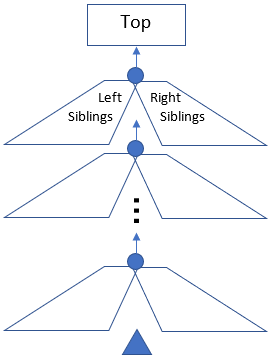
\includegraphics[width=0.6\textwidth]{figure/zipper}
\end{figure}
\end{column}
\begin{column}{0.3\textwidth}
\begin{figure}
\centering

\includegraphics[width=0.7\textwidth]{figure/real_zipper}
\end{figure}
\end{column}
\end{columns}

\end{frame}
%%%% end [tree] %%%%

%%%% begin [tree] %%%%
\begin{frame}[fragile]
\frametitle{Huet's Zipper}

\newcommand{\AS}[1]{\textcolor{red}{#1}}
\newcommand{\AL}[1]{\textcolor{blue}{#1}}

\begin{itemize}
\item For ordered trees with \AL{payload only on leaves}:

\begin{itemize}
\item
\begin{lstlisting}
'a tree = <@\AL{Leaf 'a}@> | Node <@\AL{\sout{'a}}@> ('a tree list)
\end{lstlisting}
\end{itemize}

\item Focus on a \AS{subtree} instead of an element

\begin{itemize}
\item
\begin{lstlisting}
'a tree_pointer = <@\AS{\sout{'a} \underline{'a tree}}@> * 'a tree_context
\end{lstlisting}

\item 
\begin{lstlisting}
'a tree_context = <@\AS{\sout{'a tree list *}}@> 'a tree_ancestors
\end{lstlisting}

\item 
\begin{lstlisting}
'a tree_ancestors =
    Top
  | IsChild ('a tree list) <@\AL{\sout{'a}}@> ('a tree list)
            ('a tree_ancestors)
\end{lstlisting}

\end{itemize} 

\end{itemize}
\end{frame}


\section{Context as a Derivative}

\begin{frame}[fragile]
\frametitle{Context Examples Recap}

\begin{itemize}[<+->]
\item
\begin{lstlisting}
'a list = unit + 'a * 'a list
'a list_context = 'a list * 'a list
\end{lstlisting}

\item
\begin{lstlisting}
'a btree = unit + 'a * 'a btree * 'a btree
'a btree_context = 'a btree * 'a btree
           * (bool * 'a * 'a btree) list
\end{lstlisting}

\item 
\begin{lstlisting}
'a tree = unit + 'a * a tree list
'a tree_context = 'a tree list
           * ('a tree list * 'a * 'a tree list) list
\end{lstlisting}

\item Math-ly notation, e.g. $\Flist (a) = 1 + a \times \Flist (a)$

\item Context for an arbitrary algebraic data type?
\end{itemize}
\end{frame}

\begin{frame}[fragile]
\frametitle{Context of Basic Types}

\begin{itemize}[<+->]
\item Note the context of type $a$ inside type $T$ by $C[a](T)$
\begin{itemize}
\item e.g. $C[a](\Flist(a)) = \Fdlist(a) = \Flist(a) \times \Flist(a)$
\end{itemize}

\item Context of type $a$ inside type $1$ (i.e. \lstinline|unit|): impossible!
\begin{itemize}
\item $C[a](1) = 0$
\end{itemize}

\item Context of type $a$ inside type $a$: dummy unit
\begin{itemize}
\item $C[a](a) = 1$
\end{itemize}
\end{itemize}
\end{frame}

\begin{frame}
\frametitle{Context of Sum Type}
\begin{itemize}
\item Inside $T_1 + T_2$, type $a$ occurs in either of them
\begin{itemize}
\item $C[a](T_1+T_2) = C[a](T_1) + C[a](T_2)$
\end{itemize}
\end{itemize}

\begin{figure}
\centering

\includegraphics[width=\textwidth]{figure/sum}
\end{figure}
\end{frame}

\begin{frame}
\frametitle{Context of Product Type}
\begin{itemize}
\item Inside $T_1 \times T_2$, type $a$ occurs in one of them,
while the other must be carried in the context
\begin{itemize}
\item $C[a](T_1\times T_2) = C[a](T_1)\times T_2 + T_1\times C[a](T_2)$
content
\end{itemize}
\end{itemize}

\begin{figure}
\centering
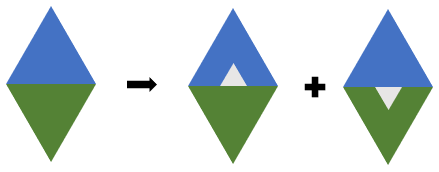
\includegraphics[width=\textwidth]{figure/prod}
\end{figure}
\end{frame}

\begin{frame}
\frametitle{Context of Composed Type}

\begin{itemize}
\item Inside composed type $T(U(a))$, type $a$ occurs in one of $U$,
which resides somewhere in $T$
\begin{itemize}
\item $C[a](T(U(a))) = C[b](T(b))|_{b=U(a)} \times  C[a](U(a))$
\end{itemize}
\end{itemize}

\begin{figure}
\centering
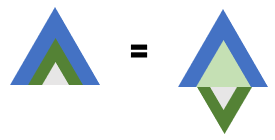
\includegraphics[width=0.7\textwidth]{figure/comp}
\end{figure}
\end{frame}

\begin{frame}
\frametitle{Context as Derivative}
\begin{itemize}
\item Rules for context:
\begin{itemize}
\item $C[a](1) = 0$
\item $C[a](a) = 1$
\item $C[a](T_1 + T_2) = C[a](T_1) + C[a](T_2)$
\item $C[a](T_1 \times  T_2) = C[a](T_1)\times T_2 + T_1\times C[a](T_2)$
\item $C[a](T(U(a))) = C[b](T(b))|_{b=U(a)} \times  C[a](U(a))$
\end{itemize}

\item Rules for derivative:
\begin{itemize}
\item $\frac{\partial}{\partial x}c = 0$
\item $\frac{\partial}{\partial x}x = 1$
\item $\frac{\partial}{\partial x}(f+g) = \frac{\partial}{\partial x}f + \frac{\partial}{\partial x}g$
\item $\frac{\partial}{\partial x}(f\cdot g) = \frac{\partial}{\partial x}f \cdot g
+ f \cdot \frac{\partial}{\partial x}g$
\item $\frac{\partial}{\partial x}(f\circ g)|_{x_0} =
\frac{\partial}{\partial u}f|_{u=g(x_0)}
\cdot \frac{\partial}{\partial x}g|_{x=x_0}$
\end{itemize}

\item $\Pa (T) \triangleq C[a](T)$
\end{itemize}
\end{frame}

%%%% begin [deriv list] %%%%
\begin{frame}
\frametitle{Context of List, Revisit}

\begin{align*}
\onslide<+->{\Pa \Flist(a)
&=\Pa (1+a \times \Flist(a))\\}
\onslide<+->{&=0 + \Pa (a \times \Flist(a))\\}
\onslide<+->{&=\Flist(a) + a \times \Pa \Flist(a)\\}
\onslide<+->{\Pa \Flist(a) &= \Flist(a) \times \Flist(a)\\}
\onslide<+->{&= \Fdlist(a)}
\end{align*}
\end{frame}
%%%% end [deriv list] %%%%

%%%% begin [deriv btree] %%%%
\begin{frame}
\frametitle{Binary Tree Context Revisit}

\begin{align*}
\onslide<+->{\Pa \Fbtree(a)
&= \Pa (1 + a \times \Fbtree^2(a)) \\}
\onslide<+->{
&=0
+ \Pa (a \times \Fbtree^2(a)) \\}
\onslide<+->{
&=\Fbtree^2(a)
+ a \times \Pa \Fbtree^2(a) \\}
\onslide<+->{
&=\Fbtree^2(a)
+ a \times 2 \times \Fbtree(a) \times \Pa \Fbtree(a) \\}
\onslide<+->{\Pa \Fbtree(a)
&= \Fbtree^2(a) \times \Flist (2 \times a \times \Fbtree(a)) \\}
\onslide<+->{
&= \Fdbtree(a)}
\end{align*}
\end{frame}
%%%% end [deriv btree] %%%%

%%%% begin [deriv tree] %%%%
\begin{frame}
\frametitle{Context of Tree, Revisit}
\begin{align*}
\onslide<+->{\Pa\Ftree(a)
&= \Pa(1 + a \times \Flist(\Ftree(a)))
\\}
\onslide<+->{
&= 0 + \Pa(a \times \Flist(\Ftree(a)))
\\}
\onslide<+->{
&=  \Flist(\Ftree(a)) + a \times \Pa(\Flist(\Ftree(a)))
\\}
\onslide<+->{
&= \Flist(\Ftree(a)) + a \times \Flist^2(\Ftree(a)) \times \Pa(\Ftree(a))
\\}
\onslide<+->{\Pa \Ftree(a)
&= \Flist(\Ftree(a)) \times \Flist(a \times \Flist^2(\Ftree(a)))
\\}
\onslide<+->{
&= \Fdtree(a)
\\}
\end{align*}
\end{frame}
%%%% end [deriv tree] %%%%

%%%% begin [deriv ltree] %%%%
\begin{frame}
\frametitle{Huet's Zipper, Revisit}

\begin{itemize}
\item $\Fltree(a) = a + \Flist(\Fltree(a))$
\item Differentiating against non-basic type is a bit tricky
\item $\frac{\partial}{\partial \Fltree}(\Fltree) = 1$?
\item $\frac{\partial}{\partial \Fltree}(\Fltree) = \frac{\partial}{\partial \Fltree}(a + \Flist(\Fltree))$?
\item A hack:
$\begin{aligned}[t]
\frac{\partial}{\partial \Fltree}
&= \mathbf{((1))} + \frac{\partial}{\partial \Fltree}(
a + \Flist(\Fltree))\\
&= \mathbf{1} + \frac{\partial}{\partial \Fltree}(\Flist(\Fltree))\\
&= \mathbf{1} + \Flist^2(\Fltree) \times \frac{\partial}{\partial \Fltree}(\Fltree) \\
&= \Fdltree
\end{aligned}$
\end{itemize}
\end{frame}
%%%% end [deriv ltree] %%%%

%%%% begin [rev] %%%%
\begin{frame}
\begin{itemize}
\item $\Pa \Ftree(a) = \Flist(\Ftree(a)) \times \Flist(a \times \Flist^2(\Ftree(a)))$
\item Reversed interpretation of the recursion path:
\end{itemize}

\bigskip

\begin{columns}
\begin{column}{0.4\textwidth}
\centering
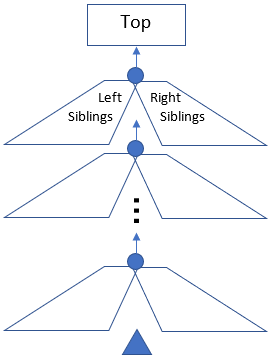
\includegraphics[width=\textwidth]{figure/zipper}
\end{column}

\begin{column}{0.4\textwidth}
\centering
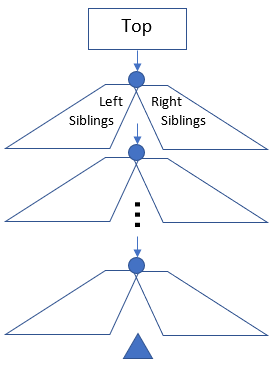
\includegraphics[width=\textwidth]{figure/zipper_rev}
\end{column}
\end{columns}
\end{frame}
%%%% end [rev] %%%%

%%%% begin [listexp] %%%%
\begin{frame}
\frametitle{Subtraction and Division?}

\begin{itemize}[<+->]
\item $\Flist(a) = 1 + a \times \Flist(a)$
\item $\Flist(a) \leftrightarrow \frac{1}{1-a}$?
\item $\Pa\Flist(a) \leftrightarrow \Pa(\frac{1}{1-a})
= \frac{1}{(1-a)^2} \leftrightarrow \Flist^2(a)$ ?!
\end{itemize}
\end{frame}
%%%% end [listexp] %%%%
\section{Combinatorial Species}

%%%% begin [species] %%%%
\begin{frame}
\frametitle{Species}

\begin{itemize}
\item General definition: endofunctor on the category of finite sets

\item Map every finite set of ``labels'' to a set of its ``arrangements''

\item Examples: $\{1, 2, 3\} \rightarrow$

\begin{itemize}
\item species of permutations:
$\big\{(1,2,3), (1,3,2), (2,3,1), \dots\big\}$
\item species of partitions:
$\Big\{\big\{\{1\},\{2\},\{3\}\big\}, \big\{\{1\}, \{2,3\}\big\}, \cdots \Big\}$
\item species of sets:
$\big\{\{1,2,3\}\big\}$
\item species of pairs:
$\{\}$
\end{itemize}

\item Species, as functors, preserve identity arrow and composition of arrows
\begin{itemize}
\item should be obvious for \textit{regular} species
\end{itemize}
\end{itemize}
\end{frame}
%%%% end [species] %%%%

%%%% begin [regular] %%%%
\begin{frame}
\frametitle{Regular Species}

\begin{itemize}
\item Composition of $0$, $1$, $X$, $+$, $\cdot$ and least fix-point
\item $0$: $\{\dots\} \rightarrow \{\}$
\item $1$: $\{\} \rightarrow \{\{\}\}$, otherwise $\{\}$
\item $X$: $\{x\} \rightarrow \{\{x\}\}$, otherwise $\{\}$
\item $F + G$: $S \rightarrow F(S) \sqcup G(S)$
\item $F \cdot G$: $S \rightarrow \bigcup\limits_{S_1 \oplus S_2=L}(F(S_1) \times G(S_2))$
\item $n \triangleq \underbrace{1 + (1 + (\ldots + 1))}_n$:
$\{\} \rightarrow \{\{\}_1, \{\}_2, \ldots, \{\}_n\}$
\item $X^n \triangleq \underbrace{X \cdot (X \cdot (\ldots \cdot X))}_n$:
$\{1, 2, \ldots, n\} \rightarrow \{\text{permutations}\}$
\item $L \triangleq 1 + X \cdot L = 1 + X \cdot (1 + X \cdot (\ldots)) \simeq 1 + X + X^2 + \ldots$
\end{itemize}
\end{frame}
%%%% end [regular] %%%%

%%%% begin [count] %%%%
\begin{frame}
\frametitle{Exponential Generating Function}

\begin{itemize}
\item Counting function: $C_F: |L| \rightarrow |F(L)|$ for species $F$
\item Exponetial Generating Function: $E_F(x) = C_F(0) + C_F(1)*\frac{x}{1!} + C_F(2)*\frac{x^2}{2!} + \ldots$
\item $E_0(x) = 0$
\item $E_1(x) = 1$
\item
$\begin{aligned}[t]
E_{F+G}(x) &= (C_F(0)+C_G(0)) + (C_f(1)+C_G(1))*\frac{x}{1!} + \ldots\\
&= E_F(x) + E_G(x)
\end{aligned}$

\item $
\begin{aligned}[t]
C_{F\cdot G}(i)*\frac{x^i}{i!} 
&= \sum\limits_{j=0}^i \frac{x^i}{i!} * \binom{i}{j}*C_F(j)*C_G(i-j)\\
&= \sum\limits_{j=0}^i \frac{x^j}{j!}*C_F(j) * \frac{x^{i-j}}{(i-j)!}*C_G(i-j)
\end{aligned}$
\item $E_{F\cdot G}(x) = E_F(x) * E_G(x)$
\item $E_F$ and $F$ share the same expression!
\end{itemize}
\end{frame}
%%%% end [count] %%%%

%%%% begin [deriv] %%%%
\begin{frame}
\frametitle{Derivative of Regular Species}

\begin{itemize}
\item $F': S \rightarrow F(S\cup\{\square\}) $
\begin{itemize}
\item e.g. $(X^2)': \{1\} \rightarrow X^2(\{1, \square\}) = \{(1,\square), (\square, 1)\}$
\end{itemize}

\item Derivative rules apply:
\begin{itemize}
\item $(F+G)'=F'+G'$
\item $(F\cdot G)' = F'\cdot G + F \cdot G'$
\item \dots
\end{itemize}

\item $(X^n)' = n * X^{n-1}$
\item $E_{(X^n)'}(x) = n * x^{n-1} = (E_{X^n}(x))'$
\item $E_{F'} = (E_F)'$
\item Derivative preserves the consistency between regular species and its counting function!
\end{itemize}
\end{frame}
%%%% end [deriv] %%%%

%%%% begin [list] %%%%
\begin{frame}
\frametitle{List, Revisit}

\begin{itemize}
\item $L = 1 + X \cdot L$
\item $E_L(x) = 1 + x \cdot E_L(x)$
\item $E_L(x) = \frac{1}{1-x}$
\item 
\begin{onlyenv}<+>
$L = \frac{1}{1 - X} = ?$
\end{onlyenv}

\item 
\begin{onlyenv}<+>
$L = \frac{1}{1 - X} = (\textbf{THE}\; F.\; E_F(x) = \frac{1}{1-x})$
\end{onlyenv}

\begin{itemize}
\item $E_F = E_G \Longrightarrow F \simeq G$ 
\end{itemize}
\end{itemize}
\end{frame}
%%%% end [list] %%%%
\section{Conclusion}

\begin{frame}
\frametitle{Conclusion}

\begin{itemize}
\item ``Functional pointer'': context type
\item The structure of context of ordered tree resembles a zipper
\item Differentiating an algebraic datatype
\item Combinatorial species and its EGF
\item Regular species vs.\ algebraic datatype?
\end{itemize}
\end{frame}
\begin{frame}[c]
\begin{center}
\Huge Thank you for listening!
\end{center}
\end{frame}
\end{document}